\section{Experimentacion}

\subsection{Herramientas de des-ensamblado}

Dedicamos este párrafo a describir las herramientas que usamos para experimentar en las próximas secciones. La herramienta que utilizamos para traducir el código de C++ a Assembler es \textit{objdump}, en base a esto podemos hacer comparaciones entre el código de C++ y Assembler. Para medir tiempos de compilación y ejecución utilizamos el comando \textit{time} y conservamos la medición de tiempo real, o sea, la correspondiente al tiempo que mide de un reloj de pared.

\subsection{Análisis del código generado}

Usando la herramienta \textit{objdump} sobre los archivos objeto (.o) del código de C++ (sin flags de optimización), obtuvimos y analizamos el código ensamblado por el compilador. Notamos las siguientes caracterísicas del código generado que dan lugar a mejoras en el rendimiento:
\begin{itemize}
	\item Dentro de la función \textit{calcVelocities}, la función donde se ralizan los cálculos que luego se vectorizarán, hay llamados a líneas consecutivas.
	\item Hay consultas a memorias innecesarias, por ejemplo, se pide un mismo valor a memoria varias veces, a pesar de haber sido guardado en un registro y nunca haber sido reemplazado con otro valor.
	\item Se manejan las variables locales almacenándolas en la pila, mientras que sólo se usan los registros de manera auxiliar para realizar operaciones.
\end{itemize}
Decidimos en consecuencia, analizar el mismo código de C++ aplicando algunas optimizaciones de compilador de GCC.
~\\

\subsection{Optimizaciones del compilador}

\subsubsection{Optimizaciones -O1}
El compilador de GCC posee una gran cantidad de optimizaciones. Un grupo de estas optimizaciones es habilitado por el parámetro -O1. Con el uso de esta optimización, el compilador se centra en reducir el tamaño del código y el tiempo de ejecución, a expensas de tiempo de compilación. Esto es comparando con la versión que no usa flags (-O0). Entre algunos de ellos se encuentran los siguientes flags:

\begin{itemize}
	\item \textit{fdce}: Realiza eliminación de código muerto en RTL \footnote{Register Transfer Language. Es una representación intermedia (RI), similar a Assembler. Se utiliza para describir el transferencia de datos de una arquitectura a nivel registro}, i.e. elimina instrucciones que no tienen efecto en la ejecución.
	\item \textit{fdse}: Realiza eliminación de guardado muerto en RTL, e.g. valores que son escritos a memoria de manera innecesaria.
	\item \textit{fmerge-constants}: Intenta unir constantes identicas (cadenas o flotantes) a través de unidades de compilación. Esta opción es la por defecto para la compilacion optimizada si el ensamblador y linker la soportan.
	\item \textit{fdelayed-branch}: No tiene efecto en el código pero causa la ejecución a priori en ramas de ejecución para aumentar la performance.
\end{itemize}

~\\
Analizamos los códigos generados por GCC con y sin flag de optimización -O1. Extrajimos la función \textit{set}, que implementa el seteo de un valor a la posición $(i, j)$ de una matriz y lo primero que notamos fue la diferencia en cantidad de las líneas de código.

\newpage

\begin{figure}[h]
\begin{center}\large{Función set de mat2}\end{center}
\begin{lstlisting}
  18e: 55                    push   rbp
  18f: 48 89 e5              mov    rbp,rsp
  192: 48 89 7d f8           mov    QWORD PTR [rbp-0x8],rdi
  196: 89 75 f4              mov    DWORD PTR [rbp-0xc],esi
  199: 89 55 f0              mov    DWORD PTR [rbp-0x10],edx
  19c: f3 0f 11 45 ec        movss  DWORD PTR [rbp-0x14],xmm0
  1a1: 48 8b 45 f8           mov    rax,QWORD PTR [rbp-0x8]
  1a5: 48 8b 10              mov    rdx,QWORD PTR [rax]
  1a8: 48 8b 45 f8           mov    rax,QWORD PTR [rbp-0x8]
  1ac: 8b 40 0c              mov    eax,DWORD PTR [rax+0xc] 
  1af: 0f af 45 f4           imul   eax,DWORD PTR [rbp-0xc]
  1b3: 89 c1                 mov    ecx,eax
  1b5: 8b 45 f0              mov    eax,DWORD PTR [rbp-0x10]
  1b8: 01 c8                 add    eax,ecx
  1ba: 48 98                 cdqe   
  1bc: 48 c1 e0 02           shl    rax,0x2
  1c0: 48 01 d0              add    rax,rdx
  1c3: f3 0f 10 45 ec        movss  xmm0,DWORD PTR [rbp-0x14]
  1c8: f3 0f 11 00           movss  DWORD PTR [rax],xmm0
  1cc: 90                    nop
  1cd: 5d                    pop    rbp
  1ce: c3                    ret    
  1cf: 90                    nop
\end{lstlisting}
\end{figure}
La versión sin opitmizar, toma los parámetros cargados en registros, los guarda en la pila y luego vuelve a cargarlos a registros distintos. Incluso realiza accesos a memoria más de una vez en busca de un mismo dato.
En cambio, la versión del código de C++ mediante la optimización, utiliza los registros para el manejo de variables locales y accede solo las veces necesarias a memoria. Este es un claro ejemplo de los efectos de los flags \textit{fdse} y \textit{fdce}.

~\\
\begin{figure}[h]
\begin{center}\large{Función set de mat2 con optimización -O1}\end{center}
\begin{lstlisting}
  d4: 0f af 77 0c           imul   esi,DWORD PTR [rdi+0xc]
  d8: 01 f2                 add    edx,esi
  da: 48 63 d2              movsxd rdx,edx
  dd: 48 8b 07              mov    rax,QWORD PTR [rdi]
  e0: f3 0f 11 04 90        movss  DWORD PTR [rax+rdx*4],xmm0
  e5: c3                    ret  
\end{lstlisting}
\end{figure}

~\\
A pesar de las mejoras que notamos con el uso de la optimización, encontramos métodos donde no se eliminaban del todo los accesos innecesarios a memoria o los fragmentos de código sin utilidad. Tomamos otro extracto de código de la función \textit{calcVelocities} (donde se realizan los cálculos más complejos) y la analizamos. 

~\\

\begin{figure}[h]
\begin{center}\large{Función calcVelocities}\end{center}
\begin{lstlisting}
  1abe:	55                   	push   rbp
  1abf:	48 89 e5             	mov    rbp,rsp
  1ac2:	48 83 ec 38          	sub    rsp,0x38
  1ac6:	48 89 7d e8          	mov    QWORD PTR [rbp-0x18],rdi
  1aca:	89 75 e4             	mov    DWORD PTR [rbp-0x1c],esi
  1acd:	89 55 e0             	mov    DWORD PTR [rbp-0x20],edx
  1ad0:	48 8b 45 e8          	mov    rax,QWORD PTR [rbp-0x18]
  1ad4:	48 8d 88 e0 00 00 00 	lea    rcx,[rax+0xe0]
  1adb:	8b 55 e0             	mov    edx,DWORD PTR [rbp-0x20]
  1ade:	8b 45 e4             	mov    eax,DWORD PTR [rbp-0x1c]
  1ae1:	89 c6                	mov    esi,eax
  1ae3:	48 89 cf             	mov    rdi,rcx
  1ae6:	e8 00 00 00 00       	call   1aeb 
  1aeb:	f3 0f 11 45 d8       	movss  DWORD PTR [rbp-0x28],xmm0
  1af0:	48 8b 45 e8          	mov    rax,QWORD PTR [rbp-0x18]
  1af4:	48 8d 88 e0 00 00 00 	lea    rcx,[rax+0xe0]
  1afb:	8b 55 e0             	mov    edx,DWORD PTR [rbp-0x20]
  1afe:	8b 45 e4             	mov    eax,DWORD PTR [rbp-0x1c]
  1b01:	89 c6                	mov    esi,eax
  1b03:	48 89 cf             	mov    rdi,rcx
  1b06:	e8 00 00 00 00       	call   1b0b 
  ...     ...      ...        ...     ...
  2400:	f3 0f 10 45 d8       	movss  xmm0,DWORD PTR [rbp-0x28]
  2405:	89 c6                	mov    esi,eax
  2407:	e8 00 00 00 00       	call   240c 
  240c:	90                   	nop
  240d:	c9                   	leave  
  240e:	c3                   	ret    
  240f:	90                   	nop
\end{lstlisting}
\end{figure}
La diferencia que notamos de los dos extractos de código de \textit{calcVelocities}, es el uso de la instrucción \textbf{nop}. El código de operación de \textbf{nop} corresponde a ``no operation'', no tiene ningun tipo de efecto, con lo cual, en el código optimizado se hace eliminación de este.
En la instrucción lad0 se carga el registro rax con un valor, no se lo pisa y luego vuelve a cargarlo en laf0. Este tipo de instrucciones donde no es necesario volver a cargar de memoria datos, vuelve a ser eliminado con el uso del flag fdse.

Volvemos a notar que en el código de C++ con flag -O1, el manejo de memoria no tiene el comportamiento de volver a cargar algo desde memoria que previamente había sido cargado y guardado en registros. Sin embargo, y apesar de las mejoras, vemos que aun repite movimientos de datos innecesarios entre registros.
Observando más detalladamente, el código con la mejora, no utiliza al máximo los registros, ya que guarda ciertos datos a memoria.

\begin{figure}[h]
\begin{center}\large{Función calcVelocities con optimización -O1}\end{center}
\begin{lstlisting}
  12f0:	41 57                	push   r15
  ...     ...                 ...    ...
  12f9:	53                   	push   rbx
  12fa:	48 83 ec 30          	sub    rsp,0x30
  12fe:	48 89 fb             	mov    rbx,rdi
  1301:	89 f5                	mov    ebp,esi
  1303:	41 89 d4             	mov    r12d,edx
  1306:	4c 8d bf e0 00 00 00 	lea    r15,[rdi+0xe0]
  130d:	4c 89 ff             	mov    rdi,r15
  1310:	e8 00 00 00 00       	call   1315
  1315:	0f 28 e0             	movaps xmm4,xmm0
  1318:	f3 0f 10 7b 1c       	movss  xmm7,DWORD PTR [rbx+0x1c]
  131d:	f3 0f 10 5b 14       	movss  xmm3,DWORD PTR [rbx+0x14]
  1322:	f3 0f 11 7c 24 04    	movss  DWORD PTR [rsp+0x4],xmm7
  1328:	0f 28 c7             	movaps xmm0,xmm7
  132b:	f3 0f 11 5c 24 10    	movss  DWORD PTR [rsp+0x10],xmm3
  1331:	f3 0f 5e c3          	divss  xmm0,xmm3
  1335:	0f 28 f0             	movaps xmm6,xmm0
  1338:	f3 0f 11 24 24       	movss  DWORD PTR [rsp],xmm4
  133d:	f3 0f 59 f4          	mulss  xmm6,xmm4
  1341:	f3 0f 11 74 24 08    	movss  DWORD PTR [rsp+0x8],xmm6
  1347:	8d 45 ff             	lea    eax,[rbp-0x1]
  134a:	44 89 e2             	mov    edx,r12d
  134d:	89 44 24 14          	mov    DWORD PTR [rsp+0x14],eax
  1351:	89 c6                	mov    esi,eax
  1353:	4c 89 ff             	mov    rdi,r15
  1356:	e8 00 00 00 00       	call   135b
  135b:	f3 0f 10 24 24       	movss  xmm4,DWORD PTR [rsp]
  ...       ...               ...     ...
  187a:	48 8d bb 30 01 00 00 	lea    rdi,[rbx+0x130]
  1881:	44 89 e2             	mov    edx,r12d
  1884:	89 ee                	mov    esi,ebp
  1886:	e8 00 00 00 00       	call   188b 
  188b:	48 83 c4 30          	add    rsp,0x30
  188f:	5b                   	pop    rbx
  ...   ...                   ...    ...
  1897:	41 5f                	pop    r15
  1899:	c3                   	ret 
\end{lstlisting}
\end{figure}
~\\

\subsubsection{Optimizaciones O2}

Las optimizaciones de -O2 realizan mejoras de velocidad y tamaño de código tal que las mejoras de una no comprometan a la otra. En comparación con -O1, aumenta aún más el tiempo de compilación y la mejora de performace del código generado.Algunos de los flags que -O2 activa son:
\begin{figure}[H]
\begin{itemize}
	\item \textit{fcse-follow-jumps}: Se eliminan códigos que se acceden mediante saltos cuya condición nunca llega a cumplirse.

	\item \textit{fgcse}: Busca instancias de expresiones idénticas (i.e. que evaluan al mismo valor) y analiza si vale la pena reemplazarlas por una única variable reteniendo el valor computado\footnote{Common Subexpression Elimination (CSE).} de manera global. También realiza constant folding\footnote{Constant folding: Evaluar expresiones constantes en tiempo de compilación.} y constant propagation \footnote{Constant propagation: Sustitución de variables por sus valores constantes en expresiones en tiempo de compilación.}.
	
  \item \textit{fgcse-lm}: Intenta reordenar instrucciones donde se produzcan sucesivas cargas/guardados que pisan valores de una misma variable. Esto permite en los loops pasar de tener una variable (registro) que se carga constantemente, a una carga fuera del loop con copias y guardados en el loop.
	
	\item \textit{finline-small-functions}: Integra el código de funciones invocadas dentro de la función que realiza el llamado, siempre que el código resultante sea menos extenso.

	\item \textit{fipa-cp}, \textit{fipa-bit-cp}, \textit{fipa-vrp}, \textit{fipa-sra}, \textit{fipa-icf}: Realizan distintos tipos de propagación de constantes y rangos, tanto en localizado como entre procedimientos.

	\item \textit{fstore-merging}: Une guardados pequeños en memoria consecutiva. Esto hace que los guardados esten bien pegaditos, ocupando menos que el tmaño de una palabraPerform merging of narrow stores to consecutive memory addresses. This pass merges contiguous stores of immediate values narrower than a word into fewer wider stores to reduce the number of instructions.

	\item \textit{ftree-tail-merge}: Busca secuencias de código idénticas, y reemplaza las repetidas con un salto a una de ellas.

	\item \textit{ftree-vrp}: Realiza Value Range Propagation en árboles. Es similar a la propagación de constantes, pero  lo hace con rangos de valores. Esto permite remover chequeos innecesarios de rangos. 
\end{itemize}
\end{figure}
Notamos varios flags que aportan a la refactorización de código, que en consecuencia, ayudan a reducir su tamaño e incluso, con ayuda de los precálculos en tiempo de compilación, reducen el tiempo de ejecución. Algunos llegan hasta el punto de modificar el orden de ejecución del código para impedir, por ejemplo, esperas por datos que no estan todavia disponibles.

~\\
Analizaremos ahora las diferencias entre el código resultado de compilar con optimizaciones -O1 y el que es generado por la compilación mediante optimizaciónes -O2. Para eso tomaremos como objeto de estudio la función \textit{setCavityFlowSpeeds}. Esta función es interesante ya que consiste de un único ciclo, dentro del cual presenta un llamado a una función con una pequeña operatoria aritmética. En particular lo que hace es recorrer el borde de cada matriz, y mediante un llamado a la función set, esta función concretamente multiplica el valor del índice \textit{i} por el valor máximo que puede tomar la variable \textit{j} y luego suma el valor de entrada de \textit{j} a este resultado, abstrayendo así el mecanismo de indexado en un arreglo plano. 

\begin{figure}[h]
\begin{center}\large{Función setCavityFlowSpeeds con optimización -O1}\end{center}
\begin{lstlisting}
  106c:   83 7f 24 00             cmp    DWORD PTR [rdi+0x24],0x0
  1070:   7e 7d                   jle    10ef
  1072:   41 56                   push   r14
  1074:   41 55                   push   r13
  1076:   41 54                   push   r12
  1078:   55                      push   rbp
  1079:   53                      push   rbx
  107a:   48 89 fd                mov    rbp,rdi
  107d:   bb 00 00 00 00          mov    ebx,0x0
  1082:   4c 8d b7 b0 00 00 00    lea    r14,[rdi+0xb0]
  1089:   4c 8d af e0 00 00 00    lea    r13,[rdi+0xe0]
  1090:   4c 8d a7 10 01 00 00    lea    r12,[rdi+0x110]
  1097:   8b 45 28                mov    eax,DWORD PTR [rbp+0x28]
  109a:   8d 50 ff                lea    edx,[rax-0x1]
  109d:   f3 0f 10 05 00 00 00    movss  xmm0,DWORD PTR [rip+0x0]
  10a4:   00 
  10a5:   89 de                   mov    esi,ebx
  10a7:   4c 89 f7                mov    rdi,r14
  10aa:   e8 00 00 00 00          call   10af
  10af:   8b 45 28                mov    eax,DWORD PTR [rbp+0x28]
  10b2:   8d 50 ff                lea    edx,[rax-0x1]
  10b5:   f3 0f 10 05 00 00 00    movss  xmm0,DWORD PTR [rip+0x0] 
  10bc:   00 
  10bd:   89 de                   mov    esi,ebx
  10bf:   4c 89 ef                mov    rdi,r13
  10c2:   e8 00 00 00 00          call   10c7
  10c7:   8b 45 28                mov    eax,DWORD PTR [rbp+0x28]
  10ca:   8d 50 ff                lea    edx,[rax-0x1]
  10cd:   f3 0f 10 05 00 00 00    movss  xmm0,DWORD PTR [rip+0x0]
  10d4:   00 
  10d5:   89 de                   mov    esi,ebx
  10d7:   4c 89 e7                mov    rdi,r12
  10da:   e8 00 00 00 00          call   10df
  10df:   83 c3 01                add    ebx,0x1
  10e2:   39 5d 24                cmp    DWORD PTR [rbp+0x24],ebx
  10e5:   7f b0                   jg     1097
  10e7:   5b                      pop    rbx
  10e8:   5d                      pop    rbp
  10e9:   41 5c                   pop    r12
  10eb:   41 5d                   pop    r13
  10ed:   41 5e                   pop    r14
  10ef:   f3 c3                   repz ret 
  10f1:   90                      nop
\end{lstlisting}
\end{figure}

~\\
\begin{figure}[h]
\begin{center}\large{Función setCavityFlowSpeeds con optimización -O2}\end{center}
\begin{lstlisting}
  1880:   44 8b 5f 24             mov    r11d,DWORD PTR [rdi+0x24]
  1884:   45 85 db                test   r11d,r11d
  1887:   7e 72                   jle    18fb
  1889:   8b 47 28                mov    eax,DWORD PTR [rdi+0x28]
  188c:   4c 63 97 bc 00 00 00    movsxd r10,DWORD PTR [rdi+0xbc]
  1893:   31 d2                   xor    edx,edx
  1895:   4c 63 8f ec 00 00 00    movsxd r9,DWORD PTR [rdi+0xec]
  189c:   4c 63 87 1c 01 00 00    movsxd r8,DWORD PTR [rdi+0x11c]
  18a3:   83 e8 01                sub    eax,0x1
  18a6:   48 98                   cdqe   
  18a8:   49 c1 e2 02             shl    r10,0x2
  18ac:   48 c1 e0 02             shl    rax,0x2
  18b0:   49 c1 e1 02             shl    r9,0x2
  18b4:   49 c1 e0 02             shl    r8,0x2
  18b8:   48 89 c6                mov    rsi,rax
  18bb:   48 89 c1                mov    rcx,rax
  18be:   48 03 b7 b0 00 00 00    add    rsi,QWORD PTR [rdi+0xb0]
  18c5:   48 03 8f e0 00 00 00    add    rcx,QWORD PTR [rdi+0xe0]
  18cc:   48 03 87 10 01 00 00    add    rax,QWORD PTR [rdi+0x110]
  18d3:   0f 1f 44 00 00          nop    DWORD PTR [rax+rax*1+0x0]
  18d8:   83 c2 01                add    edx,0x1
  18db:   c7 06 0a d7 23 3c       mov    DWORD PTR [rsi],0x3c23d70a
  18e1:   c7 01 0a d7 23 3c       mov    DWORD PTR [rcx],0x3c23d70a
  18e7:   4c 01 d6                add    rsi,r10
  18ea:   c7 00 0a d7 23 3c       mov    DWORD PTR [rax],0x3c23d70a
  18f0:   4c 01 c9                add    rcx,r9
  18f3:   4c 01 c0                add    rax,r8
  18f6:   44 39 da                cmp    edx,r11d
  18f9:   75 dd                   jne    18d8
  18fb:   f3 c3                   repz ret 
  18fd:   90                      nop
  18fe:   66 90                   xchg   ax,ax
\end{lstlisting}
\end{figure}

~\\
A grandes rasgos la optimización más notoria se constituye por un calculo previo al ciclado, de los distintos valores numéricos necesarios para luego acceder a las posiciónes de memoria necesarias. Este cálculo previo no se da en la versión -O1, sino que estos cálculos son realizados dentro del ciclo. Esto es claro ya que si observamos el ciclo que se constituye entre las lineas 1097 y 10e5 (24 instrucciónes) de la versión -O1, este consta de una mayor cantidad de líneas que el de la versión -O2, 18d8, 18f9 (9 instrucciónes). Por el contrario, el código entre el inicio de la función y el del ciclo, es más largo en la versión -O2. 

~\\
En el código mejorado con -O2 se reemplaza el uso de registros que deben ser resguardados, por registros de uso libre que no habían sido usados previamente. Esto disminuye el uso de la pila y el tiempo de accesos a memoria.\\
Los tres calls en la versión con mejora de -O1 (que por conocer la implementación de C++), corresponden al llamado de la función set para tres matrices. En la versión mejorada de -O2 se las reemplaza por el código de la función, dado que la cantidad de lineas no se vió aumentada (\textit{finline-small-functions}), de hecho disminuyó.

~\\
Además se puede notar la activación de los flags de alineamiento. Por ejemplo, se nota claramente la presencia de \textit{falign-functions}, que fuerza el comienzo de las funciones en posiciones de memoria que sean múltiplos de potencias de dos. Esto se logra insertando instrucciones sin efectos. Una forma de hacer esto es insertar líneas luego de un ret, que nunca se llegan a ejecutar. 


~\\
Si analizamos las direcciones de memoria donde se encuentran definidas las funciones, su último dígito siempre es cero. A continuación se muestran algunos ejemplos donde se ve el final de una función, con sus respectivas instrucciónes extra y el comienzo de la nueva función alineada.

~\\
\begin{figure}[h]
\begin{center}\large{calcVelocities}\end{center}
\begin{lstlisting}
  1a99:   41 5d                   pop    r13
  1a9b:   41 5e                   pop    r14
  1a9d:   c3                      ret    
  1a9e:   66 90                   xchg   ax,ax

  1aa0 <_ZN9simulator14calcVelocitiesEii>:
  1aa0:   8b 8f ec 00 00 00       mov    ecx,DWORD PTR [rdi+0xec]
  1aa6:   41 57                   push   r15
  1aa8:   41 56                   push   r14
\end{lstlisting}
\end{figure}~\\

\begin{figure}[h]
\begin{center}\large{setPBorders}\end{center}
\begin{lstlisting}
  18fb:   f3 c3                   repz ret 
  18fd:   90                      nop
  18fe:   66 90                   xchg   ax,ax

  1900 <_ZN9simulator11setPBordersEv>:
  1900:   41 56                   push   r14
  1902:   41 55                   push   r13
\end{lstlisting}
\end{figure}
Se aclara que, la potencia de dos utilizada, es algo que se especifíca en el flag cuando es utilizado por el usuario, y que no queda definida cuando este flag es agregado mediante el uso de $-$O2. Aún así el hecho de que el último dígito de todas las funciones sea cero, es un fuerte indicador de la presencia del efecto de esta optimización.\\


~\\

\subsubsection{Optimizaciones O3}

La utilización del flag -O3 aumenta aun más la cantidad de mejoras en búsqueda del aumento de la velocidad. A continuación analizamos algunos de los flags que activa.
~\\

El flag \textit{finline-functions} es similar a su correspondiente flag en -O2, \textit{finline-small-functions}, con la diferencia de que hace efecto sobre mayor cantidad de funciones. No se restringe solo a las funciones más pequeñas en cuanto a cantidad de código para mantener baja la cantidad de lineas totales.\\

En cuanto a \textit{funswitch-loops}, no hay en el programa condiciones en ciclos que sean independientes de ellos ya que todos son función de las variables sobre las que se itera. La única instancia de esto que podria darse es en la condición que decide si utilizar Assembler o C++ plano pero esta no esta escrita en el lenguaje, sino que es una directiva del compilador.\\

Tampoco se encuentran efectos de aplicar el flag \textit{fpredictive-commoning}. De aplicar, el mismo ahorarría accesos a memoria guardando datos de una iteración de un ciclo para la siguiente. No se ven ahorros de accesos a memoria ni cambios en la forma en que se accede. Tampoco se ve ningun cambio en el código al incluir el flag en una compilación realizada con -O2 y realizar una diferencia entre este y el resultado de -O2 normal.\\


\textit{ftree-partial-pre}
Por último, el flag \textit{fipa-cp-clone options} clona las funciones para realizar una sustitución de variables por sus valores constantes(i.e. \textit{constant propagation}) de forma interprocedural a un nivel aun mayor. Es altamente probable que se obtengan multiples copias de funciones, con lo cual puede incrementar el tamaño del código de manera significativa. \\

\subsection{Comparación entre secuencial, vectorial y multicore}
Ya analizado el tipo de mejoras que son implementadas por G++ al utilizar -O1, -O2 y -O3, se presentan en esta sección los resultados de los experimentos realizados. Se comparan mediciones de tiempo de los distintos flags presentes en el compilador, con otras técnicas. 
~\\
~\\
En particular se estudian los flags -O0, -O1, -O2, -O3 y -Ofast para el compilador GCC (GNU Compiler Colection), el compilador ICC (Intel C++ Compiler), para GCC+OpenMP, y por último -O0, -O3 y -Ofast para la versión vectorizada desarrollada en este trabajo, la cual consta de una parte en C++ en comun con la versión no vectorial, que fue compilada con GCC, y una función implementada en Assembler y compilada mediante NASM (Netwide Assembler x86), especificamente desarrollada para aprovechar la tecnología SIMD, y seleccionada por ser la sección mas critica en terminos de rendimiento, del programa original.
~\\
~\\
Para cada técnica se experimentó con distintos tamaños del sistema simulado, comenzando desde simulaciónes de sistemas pequeños de 1x1$m^2$ y aumentando de a un metro el lado del sistema, hasta llegar a 20x20$m^2$, el tamaño de lado es además la medida correspondiente al eje horizontal, mientras que el tiempo medido en segundos, es el correspondiente al eje vertical. Además, para cada punto, se realizaron 100 repticiónes, y se tomo la media y desvio estándar de las mismas, con el objetivo de eliminar el error de medición introducido por la falta de control del tiempo otorgado a las distintas tareas del sistema operativo por parte del scheduler. 
~\\
~\\
Los tiempos fueron medidos mediante la utilización de la herramienta time de Linux, bajo la distribución Ubuntu 16.04 LTS, en una maquina i7-920 2.67GHz, 18GB ram, 1TB HDD 7200rpm. Además no se utilizó la maquina durante la experimentación, para no introducir ruido en las mediciónes. En total se realizaron cerca de 40.000 simulaciónes. A continuación se muestran los resultados de las mismas.
~\\
~\\

\begin{figure}[!htbp]
\caption{Tiempo(s) vs Tamaño(m) para GCC}
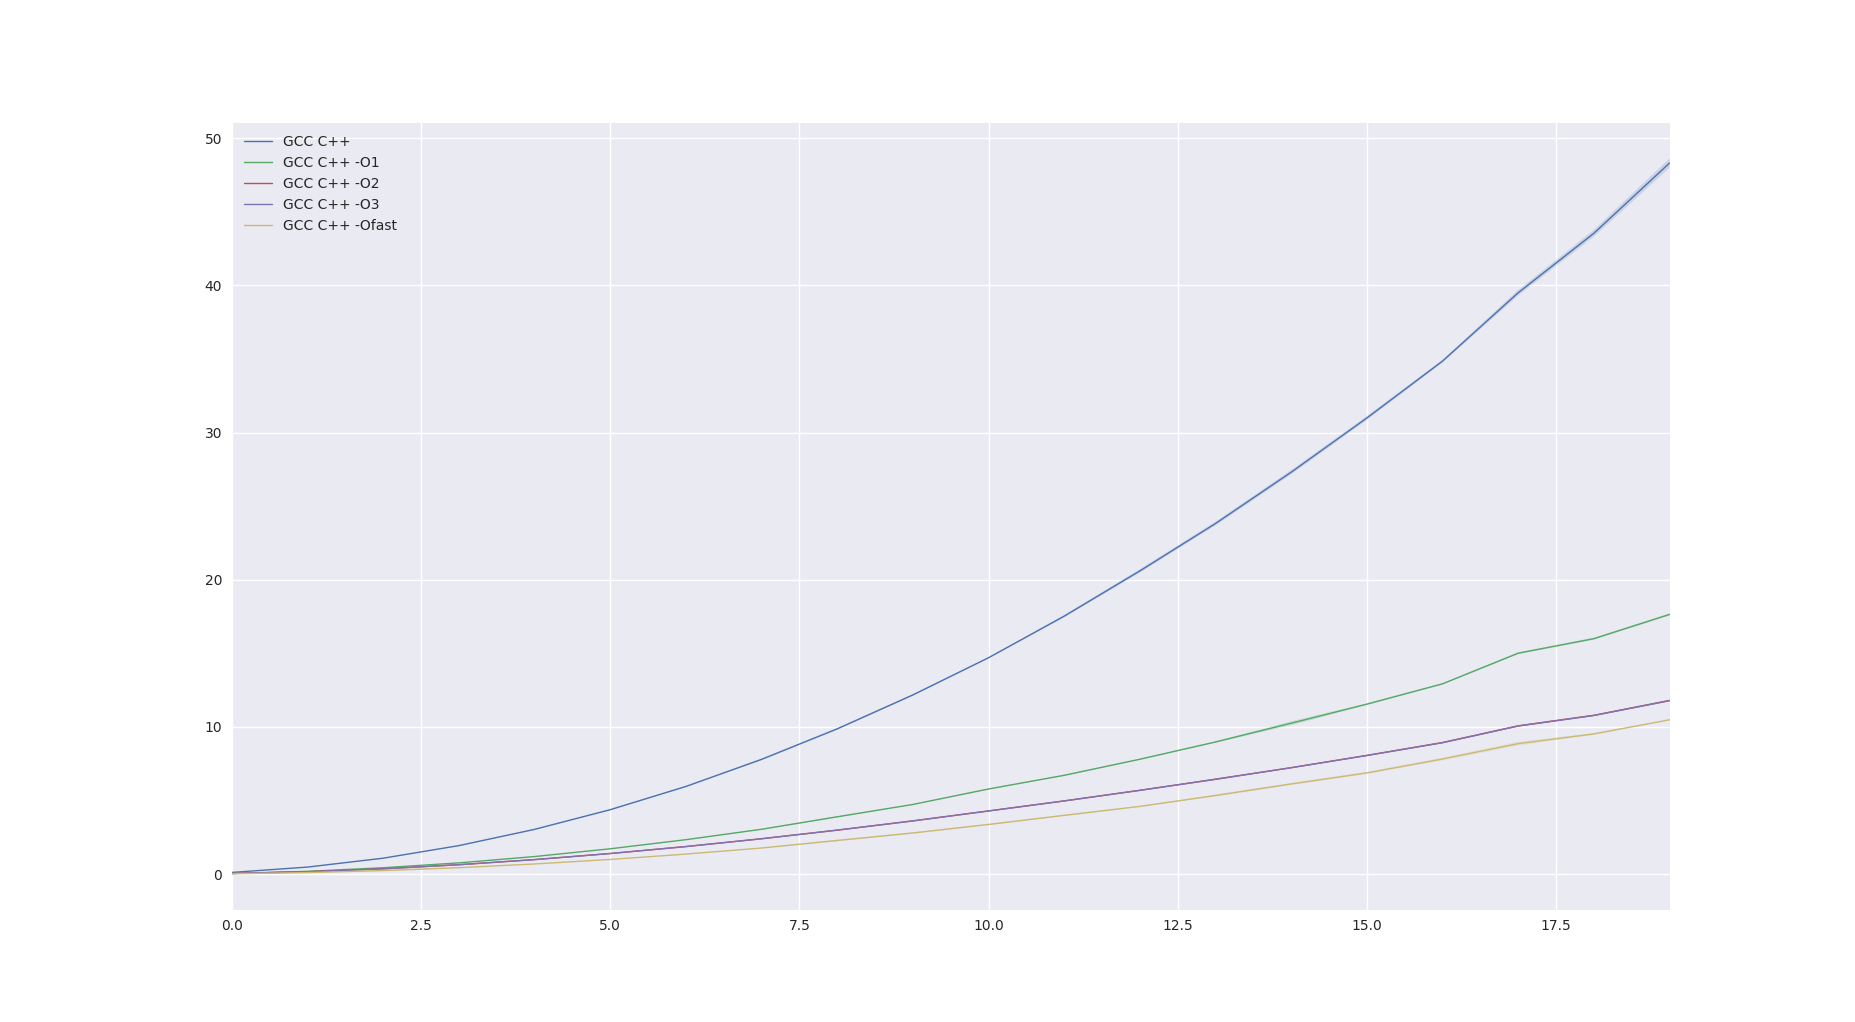
\includegraphics[width=\textwidth]{imagenes/plot_cpp.png}
\label{fig:plot_cpp}
\end{figure}

La primera experimentación consiste en el analisis de GCC, en particular su compilador C++, para distintos niveles de optimización. Esta se corresponde con la \textbf{Figura \ref{fig:plot_cpp}}.
~\\
~\\
Como es de esperar, el programa responde bien a las mejoras, con la mayor diferencia dandose entre -O0 y -O1, y la menor entre -O3 y -Ofast. Para el caso de mayor tamaño, el programa, distando de tardar casi 50s como en -O0, da un resultado menor a 20s, un tiempo menor a la mitad.
~\\
~\\
\begin{figure}[!htbp]
\caption{Tiempo(s) vs Tamaño(m) para Intel C++ Compiler}
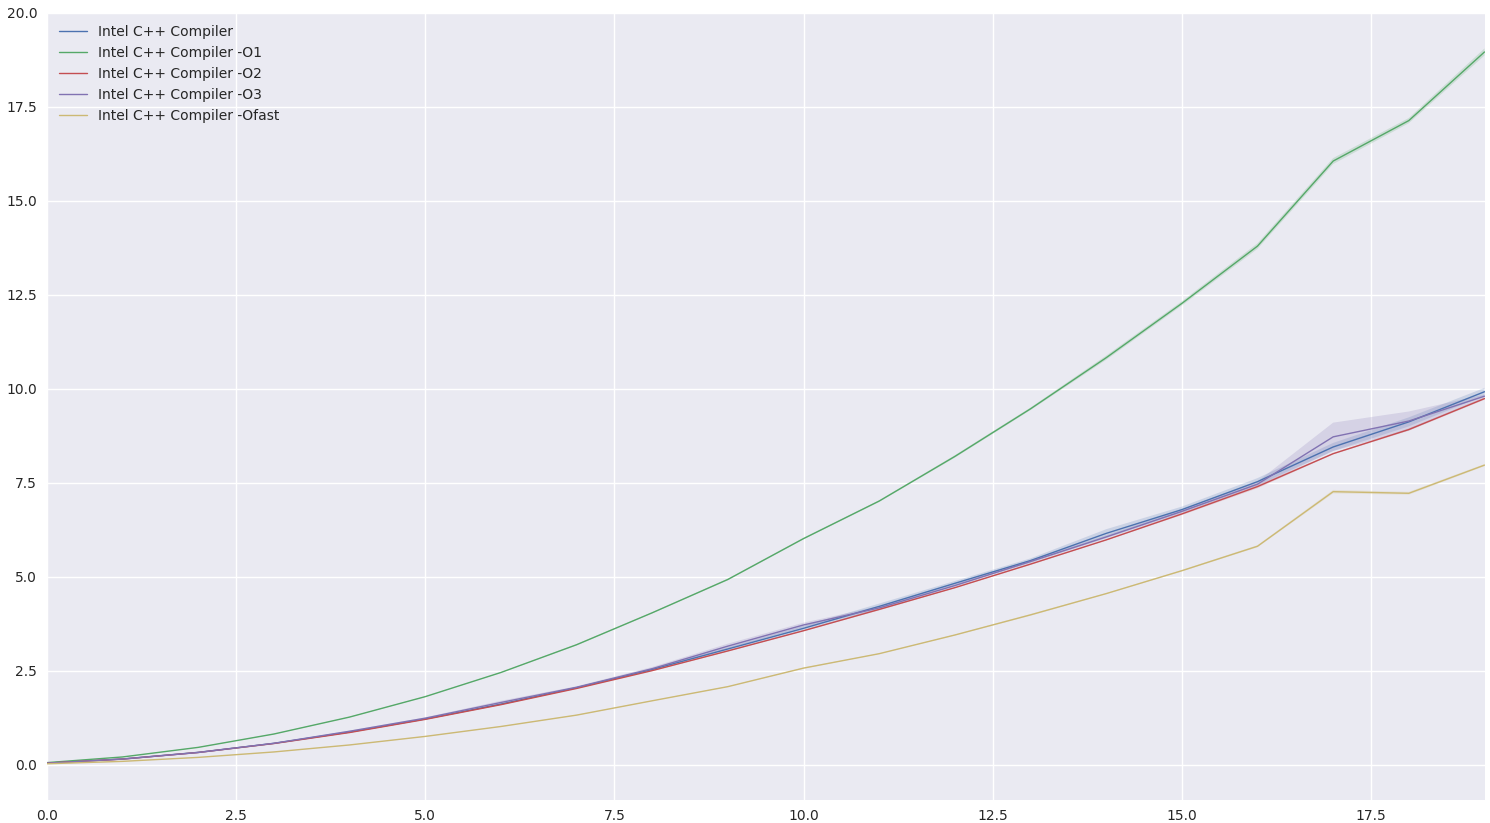
\includegraphics[width=\textwidth]{imagenes/plot_icc.png}
\label{fig:plot_icc}
\end{figure}

Donde la versión mas optimizada de GCC daba un resultado para el tamaño de 20x20m, algo menor a 20s, el compilador ICC (Intel C++ compiler), muestra en la \textbf{Figura \ref{fig:plot_icc}} un tiempo de 10s, notablemente mas rápido que  GCC -Ofast, sin utilizar optimizaciónes. Esto se debe a que este compilador, como su nombre lo indica, fue diseñado para compilar para procesadores Intel, aprovechando las características específicas de los mismos. 
~\\
~\\
Se nota aquí otra diferencia, mientras que los flags llamados -Ox en GCC implementan siempre mejoras de velocidad de ejecución, el flag -O1, en ICC, busca mejorar el tamaño del ejecutable, dando así un tiempo de ejecución mayor que al no utilizar optimizaciónes. Notar que aún así, este es mas rapido que GCC -Ofast. Finalmente, la mejor medida para ICC esta alrededor de los 8s.
~\\
~\\
\begin{figure}[!htbp]
\caption{Tiempo(s) vs Tamaño(m) para Assembler(NASM)}
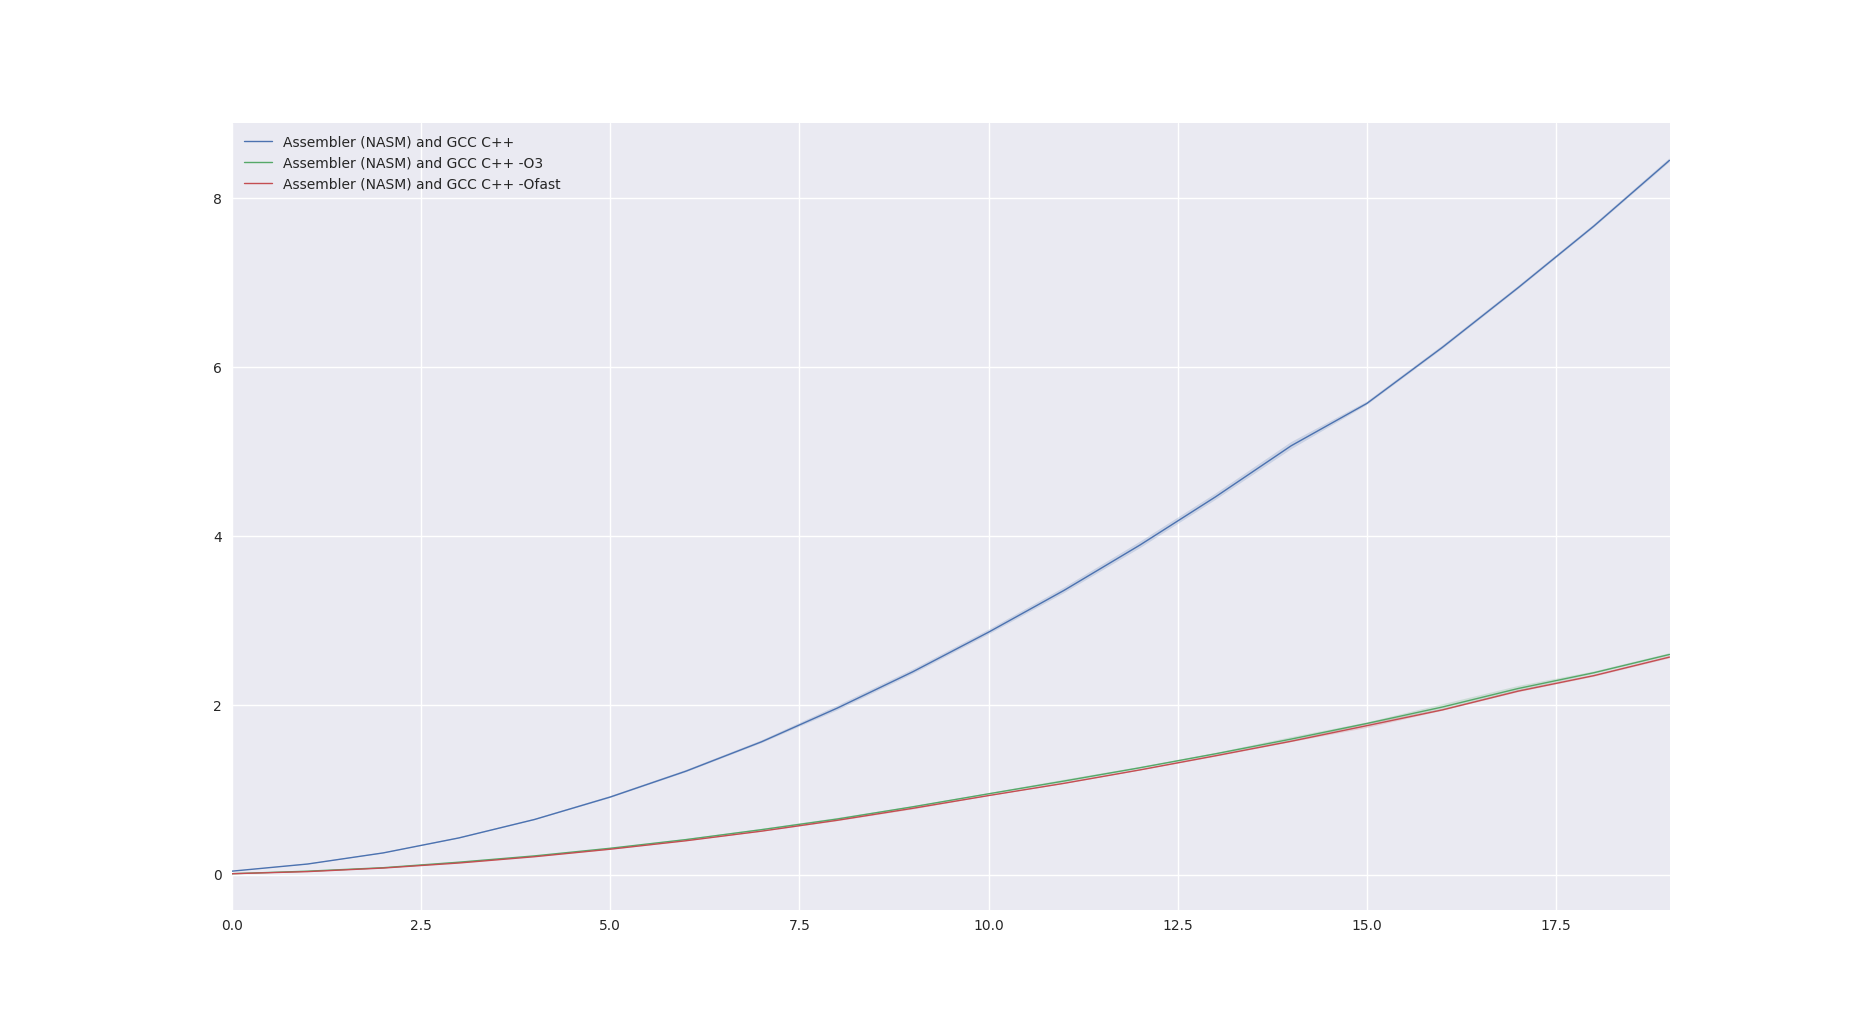
\includegraphics[width=\textwidth]{imagenes/plot_asm.png}
\label{fig:plot_asm}
\end{figure}

De la misma forma en que GCC -Ofast tenia un rendimiento similar a ICC sin optimizaciónes, la versión producida en este trabajo, aprovechando la tecnología SIMD, tiene, sin optimizaciónes, un rendimiento similar a ICC -Ofast. Esto puede verse en la \textbf{Figura \ref{fig:plot_asm}}. Tambien muestra una mejora al utilizar flags, en particular llega a un tiempo de ejecución poco mayor a 2s, al utilizar -O3 u -Ofast, optimizaciónes cuyas curvas son casi idénticas.
~\\
~\\
\begin{figure}[!htbp]
\caption{Tiempo(s) vs Tamaño(m) para GCC + OpenMP}
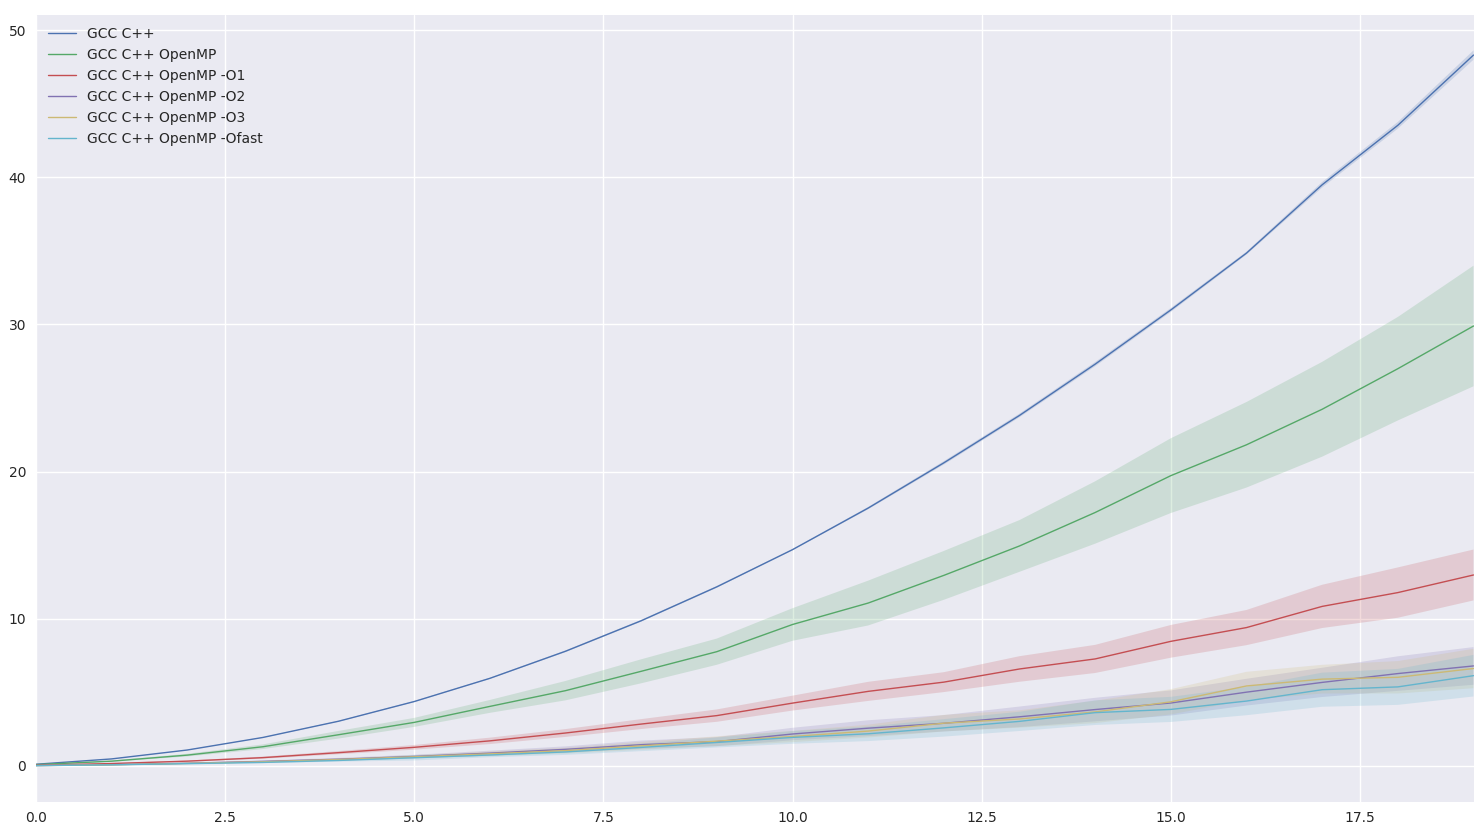
\includegraphics[width=\textwidth]{imagenes/plot_omp.png}
\label{fig:plot_omp}
\end{figure}
Otra experimentación surje de una estrategia distinta, en lugar de intentar mejorar el rendimiento mediante la optimización de codigo por si sola, se intentara hacer lo mismo mediante la asignación de mayor cantidad de recursos computacionales. OpenMP es una tecnología que logra hacer esto de forma automatica. Se dispone, mediante el mismo, de directivas que al actuar sobre un ciclo que depende de una variable, ejecuta distintas instancias del cuerpo del mismo en distintos núcleos del procesador, logrando paralelización a nivel CPU, reduciendo los tiempos de ejecición.
~\\
~\\
Los resultados correspondientes a esta experimentación, pueden verse en la \textbf{Figura \ref{fig:plot_omp}}. Una particularidad de esta gráfica, es que muestra intervalos de desviación estándar mayores que las otras. Dado que estamos agregando recursos computacionales, el uso de CPU aumenta, dejando pocos recursos para atender al resto de las tareas del sistema operativo. Se sospecha que este es el principal motivo, para el aumento drastico de la varianza de las mediciónes respecto de los otros experimentos.
~\\
~\\
Notamos que aunque la asignación de mayor cantidad de recursos aumenta significativamente el rendimiento, este no supera a la versión SIMD. Hay una explicación razonable para este fenomeno, la maquina donde se realizó la experimentación, como se comentó anteriormente, utiliza un i7-920 2.67GHz. Este modelo de procesador dispone de 4 núcleos físicos, con lo cual OpenMP puede gracias a esto, dividir la tarea en 4 partes. La versión SIMD del programa, utiliza registros XMM, y valores flotantes de 32 bits de longitud, con lo cual logra, mediante vectorización, procesar 4 puntos de la malla al mismo tiempo. Siendo que ambas técnicas procesan un maximo teórico de 4 puntos de malla por cada ejecución del cuerpo del ciclo, y que SIMD no requiere comunicación entre distintos nucleos, este resulta en mejores prestaciónes.

\begin{figure}[!htbp]
\caption{Tiempo(s) vs Tamaño(m) utilizando el flag -Ofast}
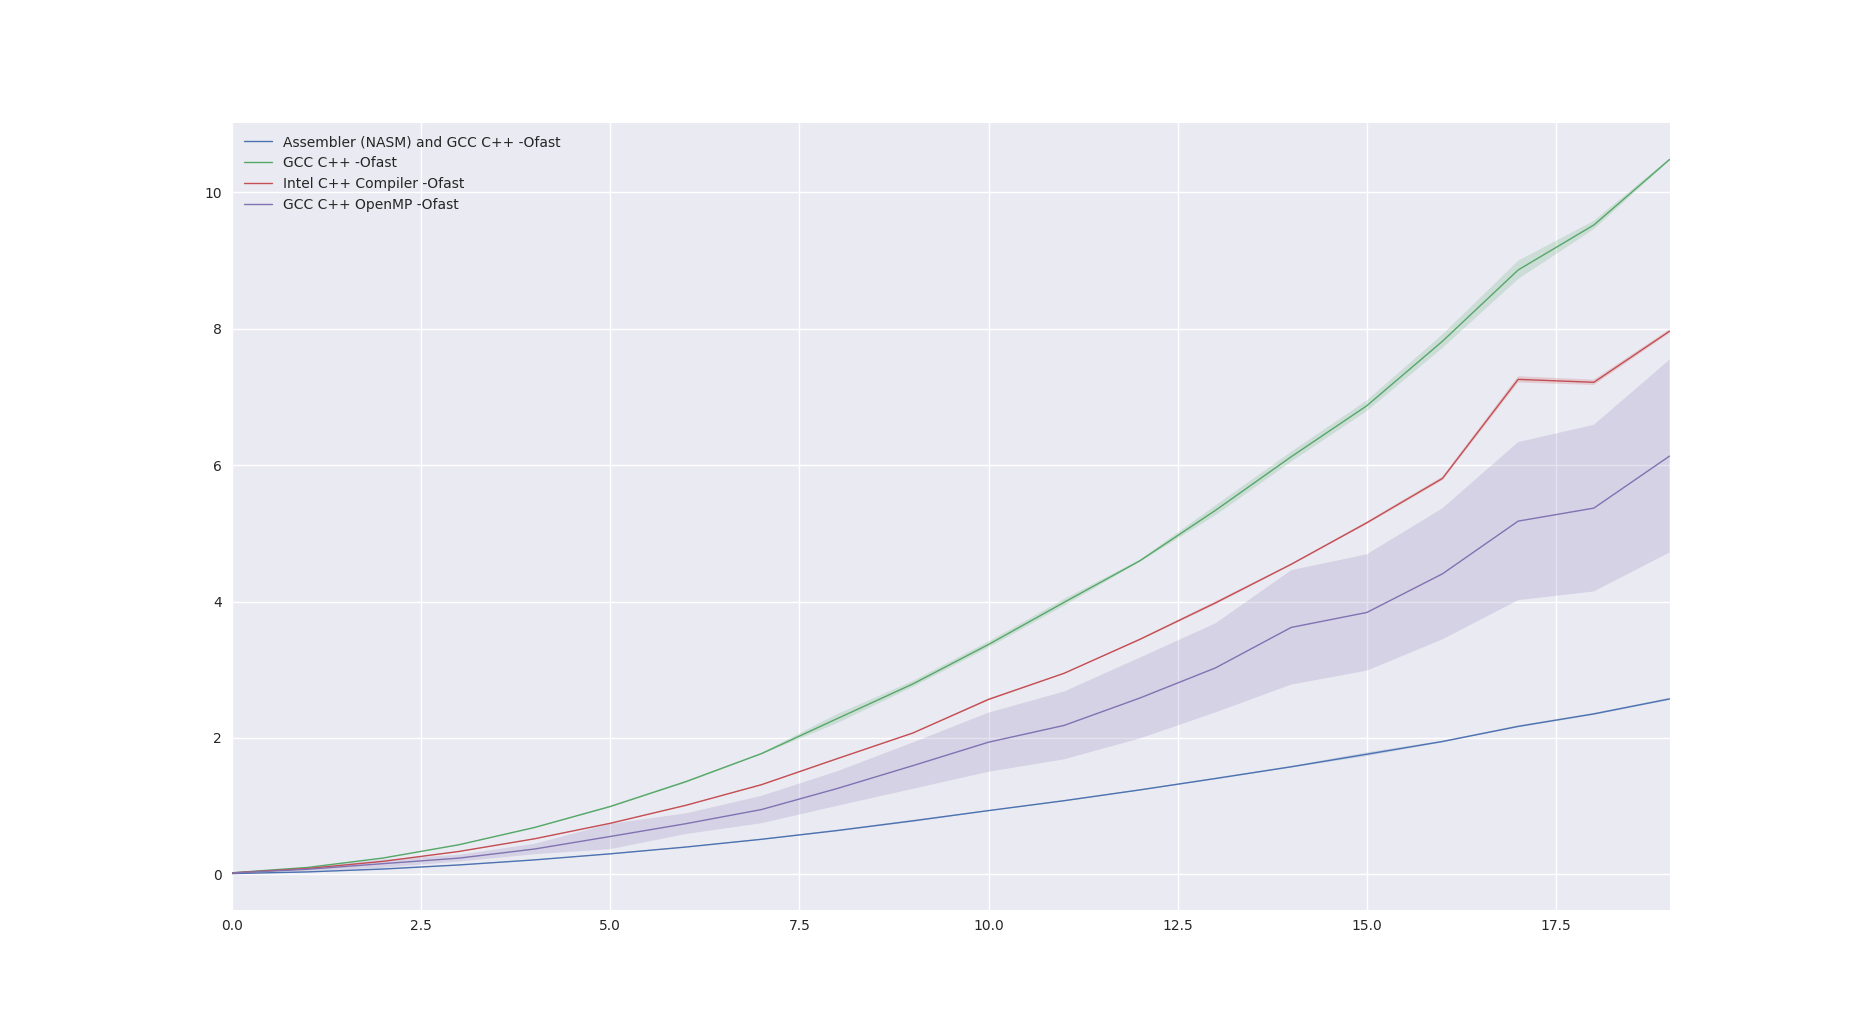
\includegraphics[width=\textwidth]{imagenes/plot_ofast.png}
\label{fig:plot_ofast}
\end{figure}
~\\
~\\

Por ultimo, y a modo ilustrativo, presentamos en la \textbf{Figura \ref{fig:plot_ofast}} una gráfica de las optimizaciónes que dieron mejor resultado para cada técnica o compilador utilizado. En todos los casos el mejor rendimiento se obtuvo mediante la utilización del flag -Ofast. Queda claro mediante esta figura, que las mejores prestaciónes se dan al utilizar SIMD, seguido por OpenMP, ICC, y finalmente GCC. El patron queda claro, mientras mas recursos se utilizen, y mas especifico sea el codigo de acuerdo a la plataforma subyacente, mejor rendimiento se obtiene. 


\subsection{CPU vs. memoria}